\documentclass[11pt,a4paper]{article}

% ---------- Page geometry: A4, 1in margins, 0.5in extra left gutter ----------
\usepackage[a4paper,top=1in,bottom=1in,right=1in,left=1.5in]{geometry}
\usepackage[utf8]{inputenc}
\usepackage[T1]{fontenc}
\usepackage{setspace}
\singlespacing

\usepackage{amsmath,amssymb}
\usepackage{graphicx}
\usepackage{tikz}
\usetikzlibrary{shapes.geometric,arrows.meta,positioning,fit,backgrounds,calc}
\usepackage{pgfgantt}
\usepackage{booktabs}
\usepackage{array}
\usepackage{longtable}
\usepackage{listings}
\usepackage{xcolor}
\usepackage{hyperref}
\hypersetup{colorlinks=true,linkcolor=blue,citecolor=blue,urlcolor=blue}
\usepackage{caption}
\usepackage{enumitem}
\usepackage{fancyhdr}
\setlength{\headheight}{14pt}

\pagestyle{fancy}
\fancyhf{}
\fancyhead[L]{ELL305 -- Computer Architecture -- Term Paper}
\fancyhead[R]{Draft 1 -- 24 August 2026}
\fancyfoot[C]{\thepage}

% ---------- listings style for the appendix ----------
\lstdefinestyle{codebox}{
  basicstyle=\ttfamily\footnotesize,
  keywordstyle=\color{blue}\bfseries,
  commentstyle=\color{gray}\itshape,
  stringstyle=\color{purple},
  numbers=left,
  numberstyle=\tiny\color{gray},
  frame=single,
  breaklines=true,
  showstringspaces=false,
  tabsize=2
}

\title{\textbf{AWS Graviton vs.\ AMD EPYC vs.\ Intel Xeon:\\
A Comparative Architecture Analysis of Modern Server Processors}\\[4pt]
\large Computer Architecture (ELL305) -- Term Paper -- Draft 1}
\author{{[}Student 1 Name{]} \\ {[}Student 2 Name{]} \\[4pt]
\small Department of Electrical Engineering \\
\small Indian Institute of Technology Delhi}
\date{24 August 2026}

\begin{document}

\maketitle

\begin{abstract}
\noindent
This document reports the progress made on the term paper titled \emph{AWS Graviton vs.\ AMD
EPYC vs.\ Intel Xeon: A Comparative Architecture Analysis of Modern Server Processors} as of
24 August 2026. Per the instructions for Draft~1, this document is a \textbf{progress report}
--- the ``Background Preparations'' expected at this stage --- and not a preliminary version of
the final $\sim$150-page term paper.

The chosen topic undertakes a comparative architectural study of three families of modern
data-centre server processors: Amazon Web Services' custom Arm-based Graviton processors,
AMD's x86-64 EPYC processors (Zen microarchitecture family), and Intel's x86-64 Xeon Scalable
processors. The comparison spans core microarchitecture, cache and memory-system design,
multicore/multiprocessor organisation, interconnect topology, and power/performance
trade-offs -- all of which map onto Chapter~12 (\emph{Multiprocessor Systems}), Chapter~11
(\emph{The Memory System}), and Appendix~A (\emph{Case Studies of Real Processors}) of the
prescribed textbook.

This draft records the selected topic, the textbook mapping, the identified work packages,
literature-survey progress so far, preliminary technical understanding, the division of work
between the two authors, a Gantt chart of progress, and the plan for subsequent cumulative
drafts. The detailed quantitative benchmarking, the full microarchitectural comparison, and the
complete literature synthesis will be developed in later submissions.

\vspace{4pt}
\noindent\textbf{Keywords:} server processors, AWS Graviton, AMD EPYC, Intel Xeon, multicore
architecture, cache coherence, memory system, Arm Neoverse, x86-64, data-centre computing
\end{abstract}

\tableofcontents
\newpage

% =====================================================================
\section{Background Preparations: Work Done as of 24 August 2026}
% =====================================================================

\subsection{Chosen Topic}
The chosen topic is \textbf{``AWS Graviton vs.\ AMD EPYC vs.\ Intel Xeon: A Comparative
Architecture Analysis of Modern Server Processors.''} The paper will compare three
production server-CPU families that currently dominate public-cloud and enterprise
data-centre compute:
\begin{itemize}[nosep]
  \item \textbf{AWS Graviton} (Graviton2/3/4) -- Amazon's custom Arm-based server SoCs, built
        on Arm Neoverse cores (N1/V1/V2), designed in-house for AWS EC2 instances.
  \item \textbf{AMD EPYC} (Zen 2 / Zen 3 / Zen 4, i.e.\ Rome / Milan / Genoa) -- AMD's
        x86-64 server processors built from chiplet-based ``Zen'' cores connected via the
        Infinity Fabric interconnect.
  \item \textbf{Intel Xeon Scalable} (Ice Lake-SP / Sapphire Rapids / Emerald Rapids) --
        Intel's x86-64 server processors, historically monolithic and more recently
        tile-based, connected via a mesh/EMIB interconnect.
\end{itemize}
The paper will study these three families along five axes: (i) core microarchitecture
(pipeline depth, issue width, branch prediction, out-of-order window), (ii) cache hierarchy
and memory system (private/shared cache sizes, coherence protocol, memory channels,
bandwidth), (iii) multicore/multiprocessor organisation (interconnect topology, chiplet vs.\
monolithic design, NUMA behaviour), (iv) ISA-level differences (Arm64/SVE vs.\ x86-64/AVX),
and (v) power, performance, and performance-per-dollar/performance-per-watt trade-offs
relevant to cloud workloads.

\subsection{Mapping to the Prescribed Textbook}
Using the Table of Contents of \emph{Basic Computer Architecture} by Smruti R.\ Sarangi
(\url{https://srsarangi.github.io/archbook/archbook.pdf}) as the guideline, the term paper
maps most closely onto the following chapters, sections, and appendix:

\begin{table}[h]
\centering
\begin{tabular}{@{}p{2.6cm}p{5.6cm}p{6.4cm}@{}}
\toprule
\textbf{Chapter} & \textbf{Title / Relevant Sections} & \textbf{Relevance to this term paper} \\
\midrule
Ch.\ 12 & \emph{Multiprocessor Systems} --
  \S12.4 MIMD Multiprocessors, \S12.4.2 Coherence, \S12.4.3 Memory Consistency,
  \S12.4.5--12.4.6 Shared/Coherent Private Caches, \S12.6 Interconnection Networks &
  \textbf{Primary chapter.} Directly covers the multicore/multi-socket organisation,
  cache-coherence, and interconnect topics (Infinity Fabric, mesh, EMIB) central to comparing
  the three processor families. \\
Ch.\ 11 & \emph{The Memory System} --
  \S11.2 Caches, \S11.3 The Memory System (bandwidth, hit/miss optimisation) &
  Needed to compare L1/L2/L3 cache sizing, memory-channel counts, and DDR5/HBM
  bandwidth across Graviton, EPYC, and Xeon. \\
Ch.\ 10 & \emph{Principles of Pipelining} --
  \S10.11 Advanced Techniques (branch prediction, multiple-issue, out-of-order pipelines) &
  Needed to compare core-level pipeline width and out-of-order execution capability
  (Neoverse V2 vs.\ Zen 4 vs.\ Golden Cove/Redwood Cove). \\
App.\ A & \emph{Case Studies of Real Processors} --
  \S A.1 ARM Processors, \S A.2 AMD Processors, \S A.3 Intel Processors &
  Directly analogous in structure to this term paper; provides the template for how to
  present a processor case study, though the specific processors discussed in the textbook
  (Cortex-A15, Bulldozer, Sandy Bridge) predate our subjects and will be updated with current
  server-class designs. \\
\bottomrule
\end{tabular}
\caption{Mapping of the term paper to the prescribed textbook.}
\end{table}

\noindent Per the course's doubt-resolution rule, since the topic is spanned by
Chapters~1--12 (primarily Chapter~12), doubts on this term paper will be routed --
after first consulting the TAs -- to \textbf{Prof.\ Sumantra DuttaRoy}.

\subsection{Why the Topic was Selected}
Server-processor design has diverged sharply over the last five years: AWS's move to a custom
Arm core (Graviton) directly challenges the traditional x86-64 duopoly of Intel and AMD, while
AMD's chiplet-based Zen architecture and Intel's more recent tile-based Sapphire Rapids design
represent two very different answers to the same scaling problem. This makes the topic a
natural, concrete vehicle for applying the multiprocessor, memory-system, and pipelining
concepts taught in ELL305 to real, publicly documented, currently-shipping hardware.

% =====================================================================
\section{Work Packages and Progress}
% =====================================================================

Following the suggested breakup in the course's Term Paper guide, work has been organised into
two work packages so far, with a third planned once the literature base is larger.

\subsection{WP1 -- Textbook Study}
\begin{itemize}[nosep]
  \item \textbf{Task 1:} Read the basic chapters titled \emph{``Chapter 11: The Memory
        System''} and \emph{``Chapter 12: Multiprocessor Systems''} from the text by
        \textbf{7 September 2026} -- \textbf{35\% done} (Chapter 11 read in full; Chapter 12
        \S12.1--\S12.4.3 read, remainder in progress).
  \item \textbf{Task 2:} Read papers related to the topic and store the references and PDFs
        in Zotero (library shared with Prof.\ Subrat Kar as per course policy)
        -- \textbf{20\% done} (5 sources logged so far; see \S\ref{sec:litsurvey}).
\end{itemize}

\subsection{WP2 -- Literature Identification and Zotero}
\begin{itemize}[nosep]
  \item \textbf{Task 3:} Cite all references read so far -- \textbf{5 references} have been
        read/skimmed and entered into the shared Zotero library to date (see the reference
        list at the end of this document).
\end{itemize}

\subsection{Papers Read So Far}
So far the following categories of sources have been identified and logged in Zotero:
architecture-vendor technical disclosures (Hot Chips talks and architecture-day materials for
Zen~4 and Sapphire Rapids), the Arm Neoverse platform documentation underlying Graviton,
and standard textbook/monograph treatments of cache coherence and memory consistency that
will anchor the theoretical framing of the paper.

\subsection{WP4 -- Preliminary Technical Study}
Alongside the literature search, the team has begun building intuition for the multicore
organisation of the three processor families using block diagrams (Figure~\ref{fig:soc-block}),
which will be refined once primary-source die photographs and vendor block diagrams have been
studied in detail.

% =====================================================================
\section{Preliminary Technical Understanding}
% =====================================================================

\subsection{Generic Multicore Server SoC Organisation}
All three processor families are, at the highest level, instances of the MIMD
shared-memory multiprocessor organisation described in Chapter~12 of the textbook: many
identical cores, each with private L1/L2 caches, sharing a last-level cache and a
memory/interconnect fabric, as sketched in Figure~\ref{fig:soc-block}.

\begin{figure}[h]
\centering
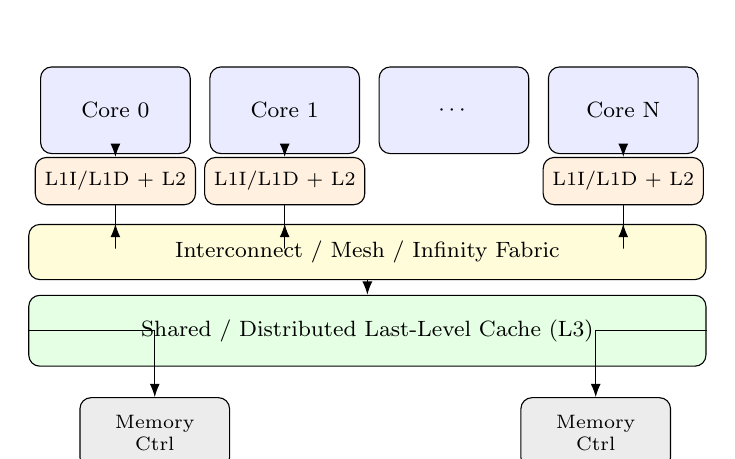
\begin{tikzpicture}[
  core/.style={draw, rounded corners, minimum width=1.9cm, minimum height=1.1cm, align=center, fill=blue!8, font=\footnotesize},
  cache/.style={draw, rounded corners, minimum width=1.9cm, minimum height=0.6cm, align=center, fill=orange!12, font=\scriptsize},
  llc/.style={draw, rounded corners, minimum width=8.6cm, minimum height=0.9cm, align=center, fill=green!10, font=\footnotesize},
  mc/.style={draw, rounded corners, minimum width=1.9cm, minimum height=0.9cm, align=center, fill=gray!15, font=\scriptsize},
  interconnect/.style={draw, rounded corners, minimum width=8.6cm, minimum height=0.7cm, align=center, fill=yellow!15, font=\footnotesize}
]

% Cores row
\foreach \i/\name in {0/Core 0,1/Core 1,2/{$\cdots$},3/Core N} {
  \node[core] (c\i) at (\i*2.15,3.0) {\name};
  \ifnum\i<2
    \node[cache, below=1pt of c\i] (l\i) {L1I/L1D + L2};
  \fi
}
\node[cache, below=1pt of c3] (l3) {L1I/L1D + L2};

% Interconnect
\node[interconnect] (ic) at (3.2,1.2) {Interconnect / Mesh / Infinity Fabric};

% LLC
\node[llc] (llc) at (3.2,0.2) {Shared / Distributed Last-Level Cache (L3)};

% Memory controllers
\node[mc] (mc1) at (0.5,-1.1) {Memory\\Ctrl};
\node[mc] (mc2) at (6.1,-1.1) {Memory\\Ctrl};

% arrows
\draw[-{Latex}] (c0) -- (l0);
\draw[-{Latex}] (c1) -- (l1);
\draw[-{Latex}] (c3) -- (l3);
\draw[-{Latex}] (l0.south) -- ++(0,-0.55) -| (ic.north -| l0);
\draw[-{Latex}] (l1.south) -- ++(0,-0.55) -| (ic.north -| l1);
\draw[-{Latex}] (l3.south) -- ++(0,-0.55) -| (ic.north -| l3);
\draw[-{Latex}] (ic) -- (llc);
\draw[-{Latex}] (llc.west) -| (mc1.north);
\draw[-{Latex}] (llc.east) -| (mc2.north);
\end{tikzpicture}
\caption{Generic block diagram of a modern multicore server SoC (applies, with different
parameters, to Graviton, EPYC, and Xeon). Each core has private L1/L2 caches; cores are
connected through a mesh-, ring-, or fabric-based interconnect to a shared/distributed L3 and
to memory controllers -- matching the MIMD shared-memory organisation of
Chapter~12, \S12.4 of the textbook.}
\label{fig:soc-block}
\end{figure}

\subsection{Key Architectural Differences Identified So Far}
Early reading has surfaced three broad points of divergence that the paper will investigate
in depth:
\begin{enumerate}[nosep]
  \item \textbf{Monolithic vs.\ chiplet/tile construction.} Intel's earlier Xeon
        generations use a single monolithic die with a 2D mesh interconnect; AMD's EPYC uses
        multiple core-complex-die (CCD) chiplets connected to a central I/O die via
        Infinity Fabric; AWS Graviton (fabricated for AWS by TSMC) has moved toward a more
        modular design in later generations as well. This maps to the interconnection-network
        material in \S12.6 of the textbook.
  \item \textbf{ISA family.} Graviton uses the Armv8/Armv9 (Arm64) ISA built on licensed
        Arm Neoverse cores, while EPYC and Xeon both use x86-64 -- a CISC ISA in the
        terminology of Chapter~1 of the textbook -- despite internally translating to
        RISC-like micro-ops.
  \item \textbf{Cache-coherence and consistency choices.} All three implement snooping- or
        directory-based variants of MESI-family coherence protocols (Chapter~12,
        \S12.4.2--\S12.4.3), but differ in LLC inclusivity/exclusivity policy and in the
        strength of the memory-consistency model exposed to software (x86-64's TSO-like
        model vs.\ Armv8's weaker default model).
\end{enumerate}
A comparison table summarising publicly disclosed parameters (core counts, cache sizes,
memory channels) will be built once the corresponding vendor architecture-day and Hot Chips
sources have been read in full; a placeholder structure for this table is shown in
Table~\ref{tab:comparison-placeholder}.

\begin{table}[h]
\centering
\small
\begin{tabular}{@{}lccc@{}}
\toprule
\textbf{Parameter} & \textbf{AWS Graviton} & \textbf{AMD EPYC} & \textbf{Intel Xeon} \\
\midrule
Core microarchitecture & Arm Neoverse (N1/V1/V2) & Zen 2/3/4 & Golden/Redwood Cove \\
ISA & Armv8.2--8.6 (Arm64) & x86-64 & x86-64 \\
Die construction & \emph{to be confirmed} & Chiplet (CCD + IOD) & Monolithic / tile-based \\
Interconnect & \emph{to be confirmed} & Infinity Fabric & 2D mesh / EMIB \\
LLC organisation & \emph{to be confirmed} & \emph{to be confirmed} & \emph{to be confirmed} \\
\bottomrule
\end{tabular}
\caption{Placeholder comparison table -- to be populated with cited, vendor-disclosed figures
once the literature survey (\S\ref{sec:litsurvey}) is further along. Values will not be
entered without a supporting citation.}
\label{tab:comparison-placeholder}
\end{table}

% =====================================================================
\section{Initial Literature Survey}
\label{sec:litsurvey}
% =====================================================================

\subsection{Literature Categories}
References are being organised in Zotero under three categories:
\begin{enumerate}[nosep]
  \item \textbf{Vendor technical disclosures} -- Hot Chips presentations and architecture-day
        material from AMD, Intel, and Arm/AWS, which are the primary source of verifiable
        microarchitectural parameters for currently-shipping parts.
  \item \textbf{Textbooks and monographs} -- for the theoretical framing of cache coherence,
        memory consistency, and pipelining (this course's textbook, plus the standard
        Sorin--Hill--Wood primer on memory consistency and coherence).
  \item \textbf{Academic and industry benchmarking studies} -- comparative performance
        studies of Graviton, EPYC, and Xeon on cloud workloads, to be added as the survey
        proceeds.
\end{enumerate}

\subsection{Preliminary Findings}
Reading so far confirms that the three families, while functionally similar at the block-diagram
level (Figure~\ref{fig:soc-block}), make substantially different trade-offs at the
interconnect and coherence-protocol level -- which is precisely the material in Chapter~12 of
the textbook, reinforcing the chapter mapping in \S1.2.

\subsection{Reference Tracking}
5 references have been read or skimmed and logged in Zotero as of this draft; the shared
library link will be provided to Prof.\ Subrat Kar as required by the course's tooling policy.
All entries currently in the bibliography of this draft are cited in the text above or in this
section.

% =====================================================================
\section{Work Division Between the Two Authors}
% =====================================================================

\subsection{Author 1 -- x86-64 Track (AMD EPYC and Intel Xeon)}
Responsible for the microarchitectural study of AMD EPYC (Zen chiplet design, Infinity
Fabric) and Intel Xeon Scalable (mesh/tile interconnect), and for the corresponding portions
of Chapters~10--12 and Appendix~A of the textbook.

\subsection{Author 2 -- Arm/Cloud-Native Track (AWS Graviton)}
Responsible for the microarchitectural study of AWS Graviton and the underlying Arm Neoverse
core family, and for the ISA-level comparison (Armv8/Armv9 vs.\ x86-64) grounded in
Chapters~1, 4, and 5 of the textbook.

\subsection{Joint Work}
The comparative benchmarking chapter, the final synthesis/conclusions, the Gantt-chart
tracking, and all Zotero reference management are being carried out jointly by both authors.

% =====================================================================
\section{Gantt Chart and Work Schedule}
% =====================================================================

\subsection{Work-Packages Schedule}
Figure~\ref{fig:gantt} shows progress against the submission milestones fixed by the course
(Draft v0.1 -- this document; v0.2, v0.3; and the final v1.0 due on the last teaching Wednesday
of the semester, 11 November 2026).

\begin{figure}[h]
\centering
\begin{ganttchart}[
    vgrid,
    hgrid,
    x unit=0.42cm,
    y unit chart=0.7cm,
    bar/.append style={fill=blue!35},
    bar progress label font=\scriptsize,
    group/.append style={fill=gray!40},
    milestone/.append style={fill=red!60},
    title height=1,
    bar height=0.55,
    bar label font=\scriptsize,
    group label font=\scriptsize\bfseries,
    title label font=\scriptsize
  ]{1}{24}
  \gantttitle{ELL305 Term Paper -- Progress Gantt Chart (Weeks, from 24 Aug 2026)}{24} \\
  \gantttitlelist{1,...,24}{1} \\
  \ganttgroup{WP1 -- Textbook Study}{1}{7} \\
  \ganttbar[progress=35]{Task 1: Read Ch.\,11--12}{1}{5} \\
  \ganttbar[progress=20]{Task 2: Papers into Zotero}{1}{7} \\
  \ganttgroup{WP2 -- Literature}{4}{12} \\
  \ganttbar[progress=15]{Task 3: Cite refs read so far}{4}{12} \\
  \ganttgroup{WP3 -- Draft Writing}{6}{20} \\
  \ganttbar{Task 4: Draft 2 (v0.2) content}{6}{11} \\
  \ganttbar{Task 5: Draft 3 (v0.3) content}{11}{16} \\
  \ganttbar{Task 6: Benchmark data collection}{9}{16} \\
  \ganttbar{Task 7: Final synthesis / v1.0}{16}{20} \\
  \ganttmilestone{Draft v0.1 (this doc)}{1} \\
  \ganttmilestone{Draft v0.2 due}{11} \\
  \ganttmilestone{Draft v0.3 due}{16} \\
  \ganttmilestone{Final v1.0 due (11 Nov 2026)}{20}
\end{ganttchart}
\caption{Progress Gantt chart, drawn natively in \LaTeX{} using \texttt{pgfgantt}, showing the
suggested WP1/WP2 breakup plus the planned WP3 (writing) work package and the four course
submission milestones.}
\label{fig:gantt}
\end{figure}

% =====================================================================
\section{Plan for Subsequent Drafts}
% =====================================================================

\subsection{Draft 2 (v0.2)}
Complete Chapter~12 reading; expand the comparison table
(Table~\ref{tab:comparison-placeholder}) with cited, vendor-disclosed parameters for all
three processor families; add a first pass at the core-microarchitecture comparison
(pipeline width, ROB size, branch predictor).

\subsection{Draft 3 (v0.3)}
Add the cache-coherence and interconnect deep-dive (Infinity Fabric vs.\ mesh vs.\ Neoverse
CMN), incorporate at least one comparative benchmarking study, and begin drafting the
performance-per-watt / performance-per-dollar analysis relevant to cloud deployment.

\subsection{Final Submission (v1.0)}
Consolidate all corrected content from Drafts~1--3, complete the quantitative comparison and
conclusions, and finalise the BibTeX bibliography exported from Zotero.

% =====================================================================
\section{Conclusion}
% =====================================================================

As of 24 August 2026, the team has selected and scoped the topic, mapped it onto
Chapters~10--12 and Appendix~A of the prescribed textbook, identified Prof.\ Sumantra
DuttaRoy as the advisor for topic-related doubts (per the Chapters~1--12 routing rule), begun
reading the relevant textbook chapters and a small initial set of vendor and academic sources,
logged those sources in a shared Zotero library, and produced a first Gantt chart tracking
progress against the four course milestones. Subsequent drafts will progressively deepen the
microarchitectural comparison and add quantitative benchmarking data, as outlined in
Section~7.

% =====================================================================
\newpage
\begin{thebibliography}{9}

\bibitem{sarangi2025}
Smruti R. Sarangi, \emph{Basic Computer Architecture}, Version 3.09, October 2025.
\url{https://srsarangi.github.io/archbook/archbook.pdf}.

\bibitem{sorinhillwood2011}
Daniel J.\ Sorin, Mark D.\ Hill, and David A.\ Wood, \emph{A Primer on Memory Consistency and
Cache Coherence}, Synthesis Lectures on Computer Architecture, Morgan \& Claypool Publishers,
2011.

\bibitem{hennessypatterson}
John L.\ Hennessy and David A.\ Patterson, \emph{Computer Architecture: A Quantitative
Approach}, 6th edition, Morgan Kaufmann, 2019.

\bibitem{amdzen4hotchips}
AMD, \emph{4th Gen AMD EPYC (``Genoa'') / Zen 4 Core and Server Architecture}, Hot Chips 34
Symposium, 2022.

\bibitem{intelsapphirerapids}
Intel Corporation, \emph{4th Gen Intel Xeon Scalable Processor (``Sapphire Rapids'')
Architecture Overview}, Intel Architecture Day / Hot Chips materials, 2022.

\end{thebibliography}

% =====================================================================
\appendix
\section{Draft 1 Submission Checklist}
% =====================================================================

\begin{itemize}[nosep]
  \item[$\square$] Single \texttt{.tex} file, compiling to a single \texttt{.pdf}
        (this document) -- no auxiliary asset files, no \texttt{.zip}.
  \item[$\square$] All diagrams (Figure~\ref{fig:soc-block}) and the Gantt chart
        (Figure~\ref{fig:gantt}) drawn inline using TikZ / \texttt{pgfgantt}.
  \item[$\square$] Section titled ``Background Preparations'' present, with chosen topic,
        chapter mapping, advisor identification, and Gantt chart, as required by the
        Head TA's instructions.
  \item[$\square$] References logged in Zotero and rendered via a \texttt{.bib}-style list
        (see bibliography above; to be exported directly from Zotero as \texttt{.bib} for the
        final v1.0 submission).
  \item[$\square$] Code/tooling notes moved to this appendix rather than the main narrative
        (Listing~\ref{lst:gantt-source} below shows the \texttt{pgfgantt} source used to
        generate Figure~\ref{fig:gantt}, included here purely for transparency/reproducibility).
\end{itemize}

\subsection*{Appendix: Gantt Chart Source (for reference)}
\begin{lstlisting}[style=codebox,caption={Excerpt of the \texttt{pgfgantt} source used to
produce Figure~\ref{fig:gantt}.},label={lst:gantt-source},language={[LaTeX]TeX}]
\begin{ganttchart}[vgrid,hgrid,x unit=0.42cm]{1}{24}
  \gantttitle{Progress Gantt Chart}{24} \\
  \ganttgroup{WP1 -- Textbook Study}{1}{7} \\
  \ganttbar[progress=35]{Task 1: Read Ch. 11-12}{1}{5} \\
  \ganttbar[progress=20]{Task 2: Papers into Zotero}{1}{7} \\
  \ganttmilestone{Draft v0.1}{1}
\end{ganttchart}
\end{lstlisting}

\subsection*{Mandatory Tooling Used}
\begin{itemize}[nosep]
  \item \textbf{Drafting:} Obsidian (notes) exported into this single \LaTeX{} source.
  \item \textbf{Diagrams:} TikZ (block diagram, Figure~\ref{fig:soc-block}).
  \item \textbf{Gantt chart:} \texttt{pgfgantt} (Figure~\ref{fig:gantt}), drawn in \LaTeX{}
        as required.
  \item \textbf{References:} Zotero, to be rendered via BibTeX for the v1.0 submission.
\end{itemize}

\end{document}
